\documentclass[aspectratio=169,10pt]{beamer}

% -------------------- Theme & styling --------------------
\usetheme{Madrid}
\usecolortheme{default}
\usefonttheme{professionalfonts}
\setbeamertemplate{navigation symbols}{}
\setbeamertemplate{footline}{%
  \leavevmode%
  \hbox{\begin{beamercolorbox}[wd=\paperwidth,ht=2.5ex,dp=1ex,right]{footline}%
    \insertframenumber\hspace{2ex}
  \end{beamercolorbox}}%
}

\definecolor{MITred}{RGB}{163,31,52}
\definecolor{Ink}{RGB}{30,34,44}
\definecolor{Panel}{RGB}{248,249,251}
\definecolor{Mid}{RGB}{115,121,132}
\definecolor{LineGray}{RGB}{203,208,217}
\definecolor{Good}{RGB}{36,132,75}
\definecolor{Bad}{RGB}{188,54,54}
\definecolor{MethodBlue}{RGB}{45,103,190}
\definecolor{Warm}{RGB}{242,173,68}

\setbeamercolor{normal text}{fg=Ink,bg=white}
\setbeamercolor{title}{fg=white,bg=MITred}
\setbeamercolor{frametitle}{fg=white,bg=MITred}
\setbeamercolor{structure}{fg=MITred}
\setbeamercolor{block title}{bg=MITred!12,fg=Ink}
\setbeamercolor{block body}{bg=Panel,fg=Ink}
\setbeamercolor{itemize item}{fg=MITred}
\setbeamercolor{itemize subitem}{fg=MITred!80}
\setbeamercolor{footline}{fg=Mid,bg=white}
\setbeamerfont{frametitle}{series=\bfseries,size=\large}
\setbeamerfont{title}{series=\bfseries,size=\LARGE}
\setbeamerfont{subtitle}{size=\large}
\setlength{\parskip}{2pt}

% -------------------- Packages --------------------
\usepackage{amsmath,amssymb,bm}
\usepackage{booktabs}
\usepackage{graphicx}
\usepackage{tikz}
\usetikzlibrary{arrows.meta,positioning,shapes.geometric,calc}
\usepackage{siunitx}
\usepackage{multicol}
\usepackage{makecell}
\usepackage[most]{tcolorbox}

% -------------------- Macros --------------------
\newcommand{\R}{\mathbb{R}}
\newcommand{\E}{\mathbb{E}}
\newcommand{\Cov}{\operatorname{Cov}}
\newcommand{\Corr}{\operatorname{Corr}}
\newcommand{\Var}{\operatorname{Var}}
\newcommand{\MV}{\mathrm{MV}}
\newcommand{\AV}{\mathrm{AV}}
\newcommand{\argmin}{\mathop{\mathrm{arg\,min}}}
\renewcommand{\L}{\mathcal{L}}
\renewcommand{\H}{\mathcal{H}}
\renewcommand{\P}{\mathcal{P}}
\newcommand{\C}{\mathcal{C}}
\newcommand{\V}{\mathcal{V}}

\newif\ifshowfigs
\showfigstrue
\newcommand{\figurebool}[1]{\ifshowfigs#1\fi}

\newcommand{\statcard}[3]{%
  \begin{tcolorbox}[enhanced,colback=#1!7,colframe=#1!70!black,
    boxrule=0.7pt,arc=1.5mm,left=2mm,right=2mm,top=1.5mm,bottom=1.5mm]
    \centering
    {\Large\bfseries #2}\\[-0.3mm]
    {\scriptsize #3}
  \end{tcolorbox}
}

\newcommand{\metriccard}[4]{%
  \begin{tcolorbox}[enhanced,colback=Good!6,colframe=Good!65!black,
    boxrule=0.7pt,arc=1.5mm,left=1.5mm,right=1.5mm,top=1.2mm,bottom=1.2mm]
    \centering
    {\bfseries #1}\\[-0.2mm]
    {\small\textcolor{Bad}{#2} $\rightarrow$ \textcolor{Good!70!black}{\bfseries #3}}\\[-0.2mm]
    {\tiny #4}
  \end{tcolorbox}
}

\newcommand{\smallnote}[1]{{\footnotesize\itshape\textcolor{Mid}{#1}}}

\title[Reducing Regressivity in ML]{Reducing Regressivity in ML-based Mass Appraisal}
\subtitle{A covariance-penalty layer for assessor workflows}
\author{Nicol\'as Acevedo$^*$ \and Haihao Lu$^\dagger$}
\date{\today}

\begin{document}

% ==========================================================
% Slide 1
% ==========================================================
\begin{frame}[plain]
\begin{tikzpicture}[remember picture,overlay]
  \fill[MITred] (current page.south west) rectangle (current page.north east);
  \fill[white,opacity=0.08] ($(current page.north east)+(-4.2,-1.2)$) circle (3.1cm);
  \fill[white,opacity=0.07] ($(current page.south west)+(2.7,1.5)$) circle (2.0cm);
\end{tikzpicture}
\vspace{9mm}
{\color{white}
\begin{center}
{\LARGE\bfseries Reducing Regressivity in ML-based Mass Appraisal}\\[2mm]
{\large A covariance-penalty layer for assessor workflows}\\[8mm]
{\normalsize Nicol\'as Acevedo$^*$ \quad Haihao Lu$^\dagger$}\\[2mm]
{\footnotesize $^*$Operations Research Center, MIT \quad $^\dagger$Sloan School of Management, MIT}\\[11mm]
\begin{minipage}{0.72\linewidth}
\centering
{\large Better predictive ML can worsen vertical equity. A lightweight penalty recovers most of the gap while preserving accuracy.}
\end{minipage}
\end{center}}
\end{frame}

% ==========================================================
% Part I
% ==========================================================
\section{Why the problem matters}

% ----------------------------------------------------------
% Slide 2
% ----------------------------------------------------------
\begin{frame}{Why property valuation matters}
\begin{columns}[T,onlytextwidth]
\column{0.52\textwidth}
\uncover<1->{\statcard{MITred}{72\%}{of U.S. local tax revenue comes from property taxes}}
\uncover<2->{\statcard{MethodBlue}{47\%}{of local own-source general revenue}}
\uncover<3->{\statcard{Good}{\$500B}{raised each year for local public services}}

\column{0.44\textwidth}
\centering
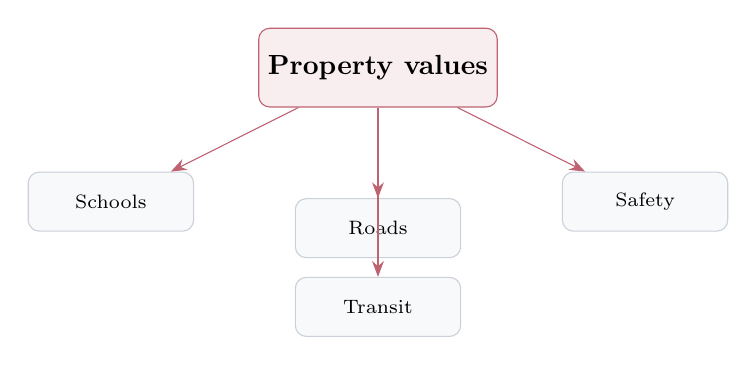
\begin{tikzpicture}[node distance=1.15cm]
  \node[draw=MITred!70,fill=MITred!8,rounded corners,minimum width=3.0cm,minimum height=1.0cm,font=\bfseries] (tax) {Property values};
  \node[draw=LineGray,fill=Panel,rounded corners,below left=of tax,minimum width=2.1cm,minimum height=0.75cm,font=\scriptsize] (schools) {Schools};
  \node[draw=LineGray,fill=Panel,rounded corners,below=of tax,minimum width=2.1cm,minimum height=0.75cm,font=\scriptsize] (roads) {Roads};
  \node[draw=LineGray,fill=Panel,rounded corners,below right=of tax,minimum width=2.1cm,minimum height=0.75cm,font=\scriptsize] (safety) {Safety};
  \node[draw=LineGray,fill=Panel,rounded corners,below=2.15cm of tax,minimum width=2.1cm,minimum height=0.75cm,font=\scriptsize] (transit) {Transit};
  \draw[-{Stealth[length=2mm]},MITred!70] (tax) -- (schools);
  \draw[-{Stealth[length=2mm]},MITred!70] (tax) -- (roads);
  \draw[-{Stealth[length=2mm]},MITred!70] (tax) -- (safety);
  \draw[-{Stealth[length=2mm]},MITred!70] (tax) -- (transit);
\end{tikzpicture}
\vspace{3mm}

\smallnote{Assessment quality is not only a prediction problem; it shapes who bears the local tax burden.}
\end{columns}
\end{frame}

% ----------------------------------------------------------
% Slide 3
% ----------------------------------------------------------
\begin{frame}{Valuation is upstream of the tax bill}
\centering
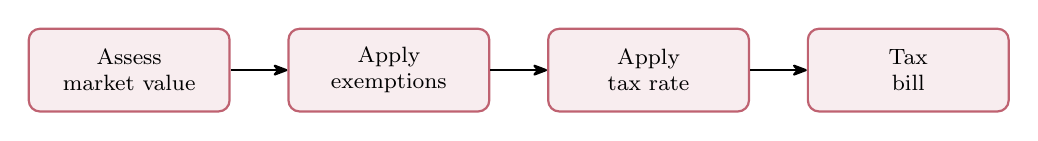
\begin{tikzpicture}[>={Stealth[round]},thick,
  node/.style={rectangle,rounded corners,draw=MITred!70,fill=MITred!8,
               minimum width=2.55cm,minimum height=1.05cm,align=center,font=\footnotesize}]
  \uncover<1->{\node[node] (A) {Assess\\market value};}
  \uncover<2->{\node[node,right=0.72cm of A] (B) {Apply\\exemptions};}
  \uncover<3->{\node[node,right=0.72cm of B] (C) {Apply\\tax rate};}
  \uncover<4->{\node[node,right=0.72cm of C] (D) {Tax\\bill};}
  \uncover<2->{\draw[->] (A) -- (B);}
  \uncover<3->{\draw[->] (B) -- (C);}
  \uncover<4->{\draw[->] (C) -- (D);}
\end{tikzpicture}

\vspace{10mm}
\begin{tcolorbox}[colback=Panel,colframe=MITred!55,width=0.78\linewidth,arc=1.5mm]
\centering
\uncover<5->{If assessed values drift by price tier, the tax burden drifts with them.}
\end{tcolorbox}
\end{frame}

% ----------------------------------------------------------
% Slide 4
% ----------------------------------------------------------
\begin{frame}{Why assessors need mass appraisal}
\begin{columns}[T,onlytextwidth]
\column{0.52\textwidth}
\centering
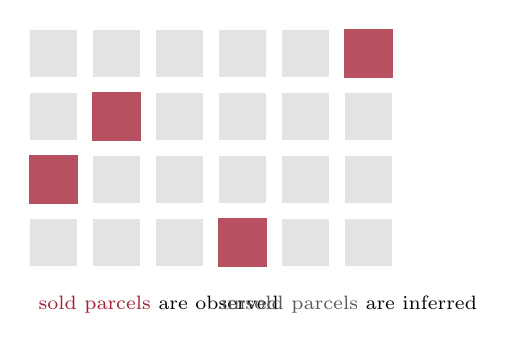
\begin{tikzpicture}[scale=0.8]
  \foreach \x in {0,...,5} {
    \foreach \y in {0,...,3} {
      \fill[gray!22] (\x,\y) rectangle ++(0.78,0.78);
      \draw[white,line width=0.8pt] (\x,\y) rectangle ++(0.78,0.78);
    }
  }
  \foreach \x/\y in {1/2,3/0,0/1,5/3} {
    \fill[MITred!78] (\x,\y) rectangle ++(0.78,0.78);
  }
  \node[font=\scriptsize,anchor=west] at (0,-0.6) {\textcolor{MITred}{sold parcels} are observed};
  \node[font=\scriptsize,anchor=west] at (2.9,-0.6) {\textcolor{gray!70!black}{unsold parcels} are inferred};
\end{tikzpicture}

\column{0.44\textwidth}
\begin{tcolorbox}[colback=MITred!6,colframe=MITred!60,arc=1.5mm]
\textbf{Mass appraisal}\\[0.5mm]
{\small Estimate many property values at a common date using common data and standardized methods.}
\end{tcolorbox}

\vspace{2mm}
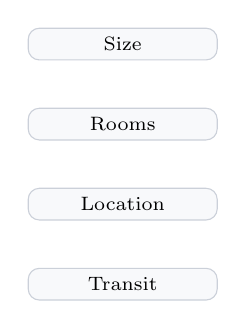
\begin{tikzpicture}[node distance=0.6cm]
  \node[draw=LineGray,fill=Panel,rounded corners,font=\scriptsize,minimum width=2.4cm] (size) {Size};
  \node[draw=LineGray,fill=Panel,rounded corners,font=\scriptsize,below=of size,minimum width=2.4cm] (rooms) {Rooms};
  \node[draw=LineGray,fill=Panel,rounded corners,font=\scriptsize,below=of rooms,minimum width=2.4cm] (loc) {Location};
  \node[draw=LineGray,fill=Panel,rounded corners,font=\scriptsize,below=of loc,minimum width=2.4cm] (transit) {Transit};
\end{tikzpicture}

\vspace{2mm}
\smallnote{Only a small share of homes transact in any year, but the full stock needs values.}
\end{columns}
\end{frame}

% ----------------------------------------------------------
% Slide 5
% ----------------------------------------------------------
\begin{frame}{Why ML is attractive here}
\begin{columns}[T,onlytextwidth]
\column{0.49\textwidth}
\begin{tcolorbox}[colback=Panel,colframe=LineGray,arc=1.5mm,title=Linear structure]
\centering
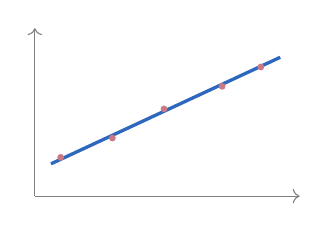
\begin{tikzpicture}[scale=0.82]
  \draw[->,gray] (0,0) -- (4.1,0);
  \draw[->,gray] (0,0) -- (0,2.6);
  \draw[MethodBlue,very thick] (0.25,0.5) -- (3.8,2.15);
  \foreach \x/\y in {0.4/0.6,1.2/0.9,2.0/1.35,2.9/1.7,3.5/2.0} {
    \fill[MITred!60] (\x,\y) circle (1.5pt);
  }
\end{tikzpicture}
\end{tcolorbox}

\column{0.49\textwidth}
\begin{tcolorbox}[colback=MethodBlue!5,colframe=MethodBlue!55,arc=1.5mm,title=Flexible tabular ML]
\centering
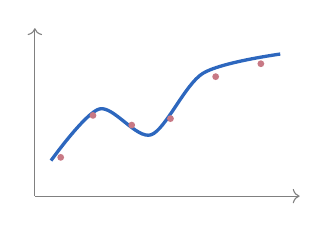
\begin{tikzpicture}[scale=0.82]
  \draw[->,gray] (0,0) -- (4.1,0);
  \draw[->,gray] (0,0) -- (0,2.6);
  \draw[MethodBlue,very thick] plot[smooth] coordinates {(0.25,0.55) (1.0,1.35) (1.8,0.95) (2.6,1.9) (3.8,2.2)};
  \foreach \x/\y in {0.4/0.6,0.9/1.25,1.5/1.1,2.1/1.2,2.8/1.85,3.5/2.05} {
    \fill[MITred!60] (\x,\y) circle (1.5pt);
  }
\end{tikzpicture}
\end{tcolorbox}
\end{columns}

\vspace{5mm}
\begin{center}
\begin{minipage}{0.76\linewidth}
\centering
Large parcel inventories, many features, and nonlinear interactions make tree-based ML useful.\\
\textbf{But predictive fit does not automatically imply equity.}
\end{minipage}
\end{center}
\end{frame}

% ----------------------------------------------------------
% Slide 6
% ----------------------------------------------------------
\begin{frame}{CCAO as the running case}
\begin{center}
\begin{tcolorbox}[colback=Panel,colframe=MITred!50,width=0.82\linewidth,arc=1.5mm]
\centering
\begin{tabular}{rl@{\hspace{1.1cm}}rl}
\textbf{Operational context} & $\sim$1.5M parcels &
\textbf{Verified sales} & 349{,}661 \\
\textbf{Features} & 95 &
\textbf{Training window} & 2016--2022 \\
\textbf{Held-out test} & 2023 &
\textbf{Validation} & 8-fold rolling origin \\
\end{tabular}
\end{tcolorbox}
\end{center}

\vspace{5mm}
\begin{columns}[T,onlytextwidth]
\column{0.31\textwidth}
\statcard{MethodBlue}{Real workflow}{CCAO residential AVM context}
\column{0.31\textwidth}
\statcard{Good}{Same diagnostics}{Ratio-study metrics assessors use}
\column{0.31\textwidth}
\statcard{Warm}{Out-of-time test}{2023 sales held out}
\end{columns}
\end{frame}

% ==========================================================
% Part II
% ==========================================================
\section{Fairness target}

% ----------------------------------------------------------
% Slide 7
% ----------------------------------------------------------
\begin{frame}{Fairness in assessment}
\begin{columns}[T,onlytextwidth]
\column{0.44\textwidth}
\begin{tcolorbox}[colback=MITred!5,colframe=MITred!60,arc=1.5mm]
\centering
\textbf{Assessment ratio}\\[-1mm]
\[
r_i=\frac{\widehat P_i}{P_i}
\]
{\small assessed value divided by sale price}
\end{tcolorbox}

\vspace{3mm}
{\small Horizontal equity asks whether similar homes have similar ratios.\\[1mm]
Vertical equity asks whether ratios are stable across value tiers.}

\column{0.53\textwidth}
\centering
\textbf{Horizontal equity}\\[-1mm]
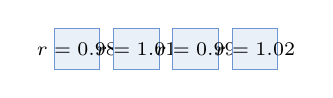
\begin{tikzpicture}[scale=0.58]
  \foreach \x/\r in {0/0.98,1.3/1.01,2.6/0.99,3.9/1.02} {
    \draw[draw=MethodBlue!70,fill=MethodBlue!10] (\x,0) rectangle ++(1.0,0.9);
    \node[font=\scriptsize] at (\x+0.5,0.45) {$r=\r$};
  }
\end{tikzpicture}

\vspace{4mm}
\textbf{Vertical equity}\\[-1mm]
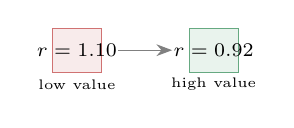
\begin{tikzpicture}[scale=0.62]
  \draw[draw=Bad!70,fill=Bad!10] (0,0) rectangle ++(1.0,0.9);
  \node[font=\scriptsize] at (0.5,0.45) {$r=1.10$};
  \node[font=\tiny] at (0.5,-0.25) {low value};
  \draw[-{Stealth[length=2mm]},gray] (1.35,0.45) -- (2.45,0.45);
  \draw[draw=Good!70,fill=Good!10] (2.8,0) rectangle ++(1.0,0.9);
  \node[font=\scriptsize] at (3.3,0.45) {$r=0.92$};
  \node[font=\tiny] at (3.3,-0.25) {high value};
\end{tikzpicture}

\vspace{2mm}
\smallnote{A downward ratio trend is regressivity.}
\end{columns}
\end{frame}

% ----------------------------------------------------------
% Slide 8
% ----------------------------------------------------------
\begin{frame}{Regressivity in taxpayer terms}
\vspace{-2mm}
\begin{columns}[T,onlytextwidth]

% -------- Q1 card --------
\column{0.47\textwidth}
\begin{tcolorbox}[enhanced,colback=Bad!5,colframe=Bad!65,arc=1.5mm,
  title=\bfseries Low-value tier (Q1),fonttitle=\small\bfseries,
  boxrule=0.6pt,left=2mm,right=2mm,top=1mm,bottom=1mm]
\centering

\begin{tikzpicture}[scale=0.42]
  \fill[Bad!25,draw=Bad!70,line width=0.6pt] (0,0) rectangle (2.2,1.5);
  \fill[Bad!45,draw=Bad!70,line width=0.6pt] (-0.25,1.5) -- (1.1,2.4) -- (2.45,1.5) -- cycle;
  \fill[white,draw=Bad!60] (0.35,0.1) rectangle (0.95,0.95);
  \fill[white,draw=Bad!60] (1.25,0.6) rectangle (1.80,1.20);
\end{tikzpicture}

\vspace{-1mm}
\small
\begin{tabular}{@{}r@{\;\;}l@{}}
Actual value    & \$144{,}491 \\
Predicted       & \$162{,}388 \\
Over-assessed   & \textcolor{Bad}{\textbf{+12.4\%}} \\[0.4mm]
\midrule
Effective rate  & \textbf{2.25\%} \\
Extra burden    & \textcolor{Bad}{\textbf{+\$358/yr}} \\
\end{tabular}
\end{tcolorbox}

% -------- arrow --------
\column{0.06\textwidth}
\centering
\vspace{22mm}
{\LARGE\color{gray!70!black}$\Longleftrightarrow$}

% -------- Q5 card --------
\column{0.47\textwidth}
\begin{tcolorbox}[enhanced,colback=Good!5,colframe=Good!65,arc=1.5mm,
  title=\bfseries High-value tier (Q5),fonttitle=\small\bfseries,
  boxrule=0.6pt,left=2mm,right=2mm,top=1mm,bottom=1mm]
\centering

\begin{tikzpicture}[scale=0.6]
  \fill[Good!25,draw=Good!70,line width=0.6pt] (0,0) rectangle (2.8,2.0);
  \fill[Good!45,draw=Good!70,line width=0.6pt] (-0.3,2.0) -- (1.4,3.1) -- (3.1,2.0) -- cycle;
  \fill[white,draw=Good!60] (0.25,0.2) rectangle (0.9,1.2);
  \fill[white,draw=Good!60] (1.2,0.2) rectangle (1.85,1.2);
  \fill[white,draw=Good!60] (2.1,0.9) rectangle (2.65,1.5);
\end{tikzpicture}

\vspace{-1mm}
\small
\begin{tabular}{@{}r@{\;\;}l@{}}
Actual value   & \$1{,}024{,}949 \\
Predicted      & \$897{,}708 \\
Under-assessed & \textcolor{Good!65!black}{\textbf{-12.4\%}} \\[0.4mm]
\midrule
Effective rate & \textbf{1.75\%} \\
Savings        & \textcolor{Good!65!black}{\textbf{-\$2{,}545/yr}} \\
\end{tabular}
\end{tcolorbox}
\end{columns}

% -------- 5-quantile strip --------
\vspace{3mm}
\begin{center}
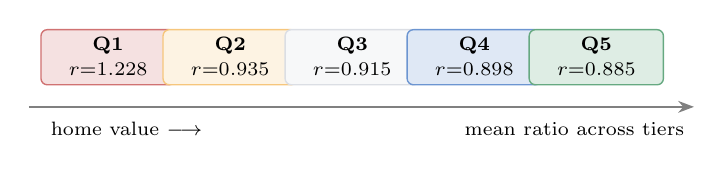
\begin{tikzpicture}[x=1.55cm,y=1cm]
  \foreach \i/\lab/\rval/\col in {0/Q1/1.228/Bad,1/Q2/0.935/Warm,2/Q3/0.915/LineGray,3/Q4/0.898/MethodBlue,4/Q5/0.885/Good} {
    \draw[fill=\col!15,draw=\col!70,rounded corners=0.8mm,line width=0.5pt] (\i,0) rectangle ++(1.1,0.7);
    \node[font=\scriptsize\bfseries] at (\i+0.55,0.50) {\lab};
    \node[font=\scriptsize] at (\i+0.55,0.20) {$r{=}\rval$};
  }
  \draw[-{Stealth[length=2mm]},thick,gray] (-0.1,-0.28) -- (5.35,-0.28);
  \node[font=\scriptsize,anchor=west] at (0,-0.56) {home value $\longrightarrow$};
  \node[font=\scriptsize,anchor=east] at (5.35,-0.56) {mean ratio across tiers};
\end{tikzpicture}
\end{center}

\vspace{2mm}
\begin{center}
\textbf{Regressive assessments shift tax burden toward lower-valued homes and away from higher-valued ones.}
\end{center}
\end{frame}

% ----------------------------------------------------------
% Slide 9
% ----------------------------------------------------------
\begin{frame}{Regressivity in diagnostic terms}
\begin{columns}[T,onlytextwidth]
\column{0.72\textwidth}
\centering
\figurebool{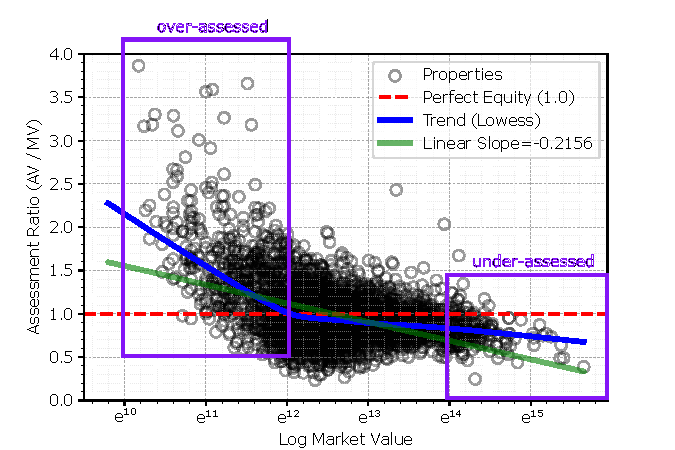
\includegraphics[width=\linewidth,trim={0 0mm 0 0}]{img/motivation/Baseline LightGBM_0_motivation_squared_only.pdf}}

\column{0.25\textwidth}
\begin{tcolorbox}[colback=Bad!6,colframe=Bad!65,arc=1.5mm]
\textbf{Diagnostic rule}\\[1mm]
{\small If $r$ declines as value rises, the model is regressive.}
\end{tcolorbox}

\vspace{3mm}
\begin{tcolorbox}[colback=Panel,colframe=LineGray,arc=1.5mm]
{\small The ratio-vs-price plot is the picture behind PRD, PRB, and VEI.}
\end{tcolorbox}
\end{columns}
\end{frame}

% ----------------------------------------------------------
% Slide 10
% ----------------------------------------------------------
\begin{frame}{The baseline tension: better ML, worse vertical equity}
\vspace{-2mm}
\begin{center}
{\small Linear Regression $\longrightarrow$ LightGBM on the CCAO 2023 held-out test set}
\end{center}

\vspace{1mm}
\begin{columns}[T,onlytextwidth]
% ---- Accuracy / horizontal equity (improves) ----
\column{0.49\textwidth}
\begin{tcolorbox}[enhanced,colback=Good!5,colframe=Good!55!black,arc=1.5mm,
  title=\bfseries Accuracy and dispersion {\normalfont\small(improve)},
  fonttitle=\small\bfseries,boxrule=0.6pt,left=2mm,right=2mm,top=1mm,bottom=1mm]
\small
\renewcommand{\arraystretch}{1.15}
\begin{tabular}{@{}l r c r c@{}}
 & \textit{LR} & & \textit{LGBM} & \\
\midrule
$R^2$     & 0.762      & $\rightarrow$ & \textbf{0.883}      & \textcolor{Good!65!black}{$\uparrow$} \\
MAE       & \$86{,}257 & $\rightarrow$ & \textbf{\$72{,}064} & \textcolor{Good!65!black}{$\downarrow$} \\
COD       & 25.0\%     & $\rightarrow$ & \textbf{23.1\%}     & \textcolor{Good!65!black}{$\downarrow$} \\
COV       & 36.8\%     & $\rightarrow$ & \textbf{35.4\%}     & \textcolor{Good!65!black}{$\downarrow$} \\
\end{tabular}
\end{tcolorbox}

% ---- Vertical equity (worsens) ----
\column{0.49\textwidth}
\begin{tcolorbox}[enhanced,colback=Bad!5,colframe=Bad!60,arc=1.5mm,
  title=\bfseries Vertical equity {\normalfont\small(worsens)},
  fonttitle=\small\bfseries,boxrule=0.6pt,left=2mm,right=2mm,top=1mm,bottom=1mm]
\small
\renewcommand{\arraystretch}{1.15}
\begin{tabular}{@{}l r c r c@{}}
 & \textit{LR} & & \textit{LGBM} & IAAO \\
\midrule
PRD & 1.039  & $\rightarrow$ & \textcolor{Bad}{\textbf{1.085}}   & $[0.98,1.03]$ \\
PRB & -0.011 & $\rightarrow$ & \textcolor{Bad}{\textbf{-0.118}}  & $[-0.05,0.05]$ \\
VEI & -13.5\%& $\rightarrow$ & \textcolor{Bad}{\textbf{-36.8\%}} & $[-10\%,10\%]$ \\
\multicolumn{5}{@{}l@{}}{\smallnote{All three metrics move outside the compliance band.}} \\
\end{tabular}
\end{tcolorbox}
\end{columns}

\vspace{4mm}
\begin{center}
\begin{tcolorbox}[enhanced,colback=Panel,colframe=MITred!55,arc=1.5mm,
  width=0.82\linewidth,boxrule=0.6pt,left=2mm,right=2mm,top=1.2mm,bottom=1.2mm]
\centering
\textbf{The stronger predictor exits the compliance region on the dimension assessors care about.}
\end{tcolorbox}
\end{center}
\end{frame}

% ==========================================================
% Part III
% ==========================================================
\section{Method}

% ----------------------------------------------------------
% Slide 11
% ----------------------------------------------------------
\begin{frame}{Main idea: add a regressivity penalty}
\begin{columns}[T,onlytextwidth]
\column{0.47\textwidth}
\begin{tcolorbox}[colback=Panel,colframe=LineGray,title=Accuracy-only learner,arc=1.5mm]
\[
\min_{f\in\H}\; L(f;X,y)
\]
\centering
{\small Optimize fit. Ignore value-dependent ratio drift.}
\end{tcolorbox}

\column{0.47\textwidth}
\begin{tcolorbox}[colback=MethodBlue!6,colframe=MethodBlue!65,title=Regressivity-aware learner,arc=1.5mm]
\[
\min_{f\in\H}\; L(f;X,y)+\rho\,\Psi
\]
\centering
{\small One knob balances accuracy and equity.}
\end{tcolorbox}
\end{columns}

\vspace{6mm}
\begin{center}

\begin{tikzpicture}[node distance=1.0cm]
  \node[draw=LineGray,fill=Panel,rounded corners,minimum width=2.8cm,minimum height=0.8cm,font=\small] (a) {Strong learner};
  \node[draw=MethodBlue!65,fill=MethodBlue!8,rounded corners,right=of a,minimum width=2.8cm,minimum height=0.8cm,font=\small] (b) {Penalty $\Psi$};
  \node[draw=Good!65,fill=Good!8,rounded corners,right=of b,minimum width=2.8cm,minimum height=0.8cm,font=\small] (c) {Tune $\rho$};
  \draw[-{Stealth[length=2mm]}] (a) -- (b);
  \draw[-{Stealth[length=2mm]}] (b) -- (c);
\end{tikzpicture}
\end{center}
\end{frame}

% ----------------------------------------------------------
% Slide 12
% ----------------------------------------------------------
\begin{frame}{Why covariance in log-space}
\centering
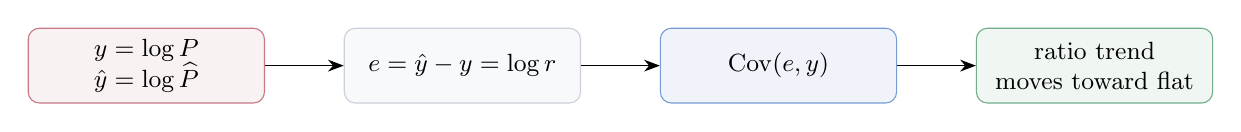
\begin{tikzpicture}[node distance=1.0cm,>={Stealth[length=2mm]},
  box/.style={draw,rounded corners,minimum width=3.0cm,minimum height=0.95cm,align=center,font=\small}]
  \node[box,fill=MITred!6,draw=MITred!60] (a) {$y=\log P$\\$\hat y=\log \widehat P$};
  \node[box,fill=Panel,draw=LineGray,right=of a] (b) {$e=\hat y-y=\log r$};
  \node[box,fill=MethodBlue!7,draw=MethodBlue!65,right=of b] (c) {$\Cov(e,y)$};
  \node[box,fill=Good!7,draw=Good!65,right=of c] (d) {ratio trend\\moves toward flat};
  \draw[->] (a) -- (b);
  \draw[->] (b) -- (c);
  \draw[->] (c) -- (d);
\end{tikzpicture}

\vspace{9mm}
\begin{tcolorbox}[colback=Panel,colframe=LineGray,width=0.74\linewidth,arc=1.5mm]
\centering
Residual drift with log-price is exactly log-ratio drift with value.
\end{tcolorbox}
\end{frame}

% ----------------------------------------------------------
% Slide 13
% ----------------------------------------------------------
\begin{frame}{Direct vs surrogate: conceptual vs operational}
\begin{columns}[T,onlytextwidth]
\column{0.48\textwidth}
\begin{tcolorbox}[colback=Panel,colframe=LineGray,title=Direct penalty,arc=1.5mm]
\textbf{Closest conceptual target}\\[1mm]
{\small Suppresses first-order dependence between log-ratios and log-prices.}\\[2mm]
{\footnotesize Best for explaining the idea.}
\end{tcolorbox}

\column{0.48\textwidth}
\begin{tcolorbox}[colback=MethodBlue!6,colframe=MethodBlue!65,title=Surrogate penalty,arc=1.5mm]
\textbf{Operational default}\\[1mm]
{\small Sample-additive, separable, and plug-and-play in LightGBM/XGBoost custom objectives.}\\[2mm]
{\footnotesize Best for routine deployment.}
\end{tcolorbox}
\end{columns}

\vspace{6mm}
\begin{center}
\textbf{Main hierarchy:} direct explains the target; surrogate is the recommended implementation.
\end{center}
\end{frame}

% ----------------------------------------------------------
% Slide 14
% ----------------------------------------------------------
\begin{frame}{Why this fits assessor workflows}
\begin{center}
\begin{tcolorbox}[colback=MethodBlue!6,colframe=MethodBlue!60,width=0.82\linewidth,arc=1.5mm]
\centering
Same preprocessing, same feature set, same base learner, same diagnostics.\\
\textbf{One added calibration knob: $\rho$.}
\end{tcolorbox}
\end{center}

\vspace{-1mm}
\begin{figure}
\centering
\figurebool{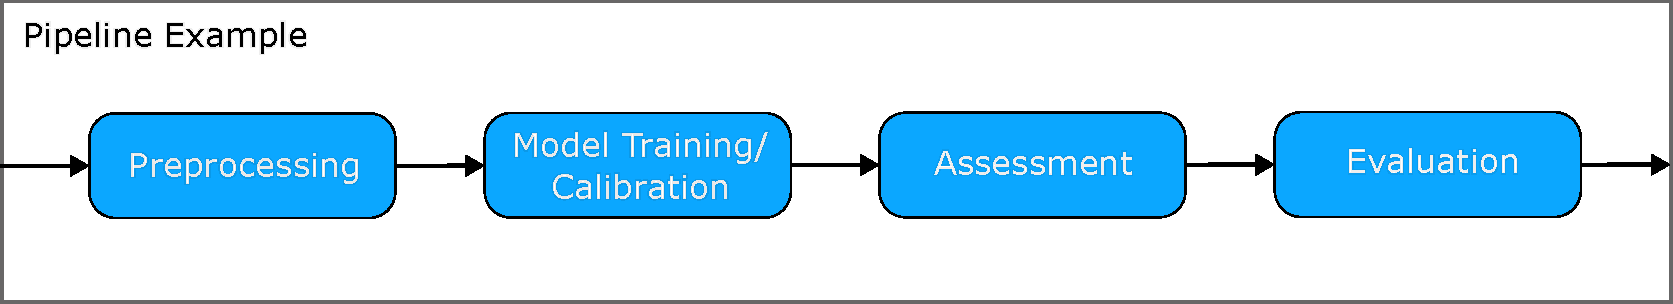
\includegraphics[width=0.80\linewidth]{img/pipeline/pipeline1.pdf}}
\end{figure}
\end{frame}

% ==========================================================
% Part IV
% ==========================================================
\section{Empirical evidence}

% ----------------------------------------------------------
% Slide 15
% ----------------------------------------------------------
\begin{frame}{Before and after: the trend flattens}
\vspace{-1mm}
\begin{columns}[T,onlytextwidth]
\column{0.49\textwidth}
\centering
{\small\textcolor{Bad}{\textbf{Baseline LightGBM}}}\\[-1mm]
\figurebool{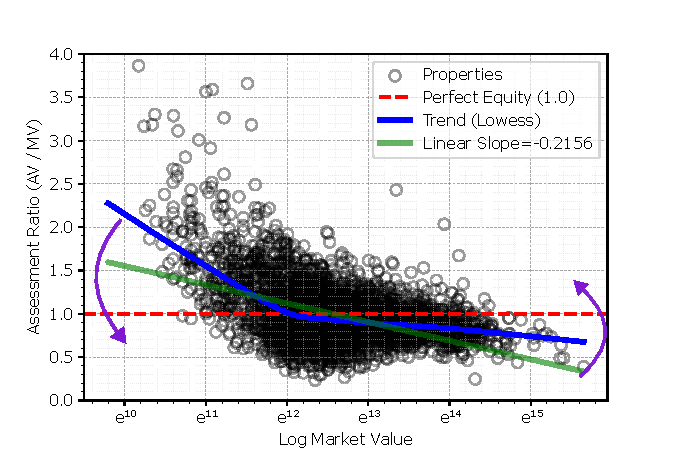
\includegraphics[width=\linewidth,trim={-1cm 0mm 1cm 3mm}]{img/motivation/Baseline LightGBM_0_motivation_arrows_3.pdf}}

\column{0.49\textwidth}
\centering
{\small\textcolor{MethodBlue}{\textbf{Penalized LightGBM}}}\\[-1mm]
\figurebool{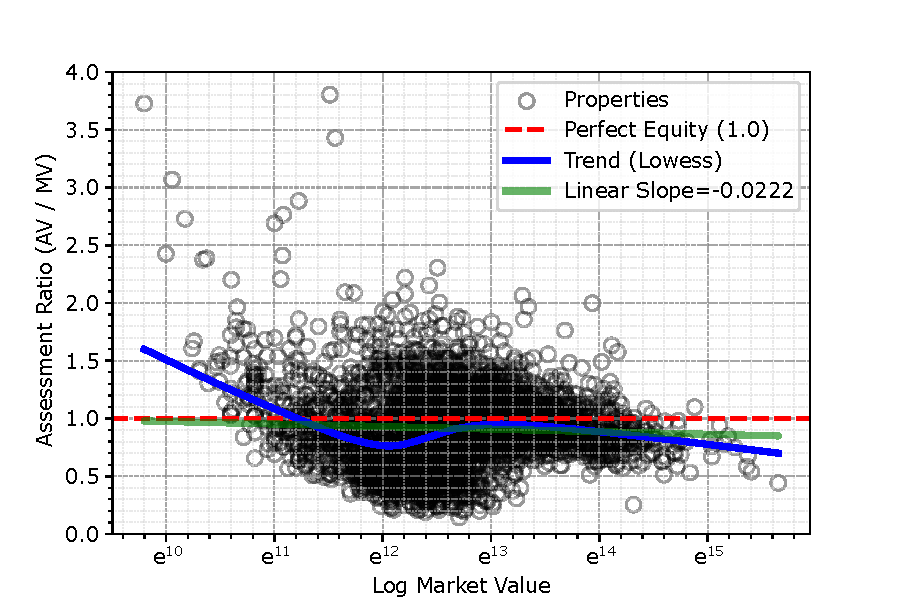
\includegraphics[width=\linewidth,trim={1cm 0mm -1cm 3mm}]{img/Covariance-Penalized LightGBM_3_motivation.pdf}}
\end{columns}

\vspace{1mm}
\begin{center}
\begin{tcolorbox}[enhanced,colback=Panel,colframe=LineGray,width=0.82\linewidth,arc=1.5mm,
  boxrule=0.6pt,left=2mm,right=2mm,top=1mm,bottom=1mm]
\centering\small
\begin{tabular}{@{}l c c c@{}}
 & Baseline & & Penalized \\
\midrule
Ratio-price correlation & \textcolor{Bad}{$-0.267$} & $\longrightarrow$ & \textcolor{MethodBlue}{$\mathbf{-0.024}$} \\
Ratio-price slope       & \textcolor{Bad}{$-0.216$} & $\longrightarrow$ & \textcolor{MethodBlue}{$\mathbf{-0.022}$} \\
\end{tabular}
\end{tcolorbox}
\end{center}
\end{frame}

% ----------------------------------------------------------
% Slide 16
% ----------------------------------------------------------
\begin{frame}{Main payoff: vertical-equity metrics recover}
\vspace{-1mm}
\begin{center}
{\small Surrogate-penalized LightGBM, $\rho=6.572$, held-out 2023 test set}
\end{center}

\vspace{2mm}
\begin{columns}[T,onlytextwidth]
\column{0.24\textwidth}
\metriccard{PRD}{1.085}{1.038}{toward $[0.98,1.03]$}
\column{0.24\textwidth}
\metriccard{PRB}{-0.118}{-0.011}{inside $[-0.05,0.05]$}
\column{0.24\textwidth}
\metriccard{VEI}{-36.8\%}{-8.5\%}{inside $[-10\%,10\%]$}
\column{0.24\textwidth}
\begin{tcolorbox}[enhanced,colback=Panel!60,colframe=Mid,boxrule=0.7pt,arc=1.5mm,
  left=1.5mm,right=1.5mm,top=1.2mm,bottom=1.2mm]
\centering
{\Large\bfseries $R^2$}\\[-0.3mm]
{\small 0.883 $\rightarrow$ \textbf{0.882}}\\[-0.2mm]
{\tiny essentially unchanged}
\end{tcolorbox}
\end{columns}

\vspace{8mm}
\begin{center}
\begin{minipage}{0.82\linewidth}
\centering
\textbf{Most of the vertical-equity gap is recovered; COD and COV also improve slightly.}\\[0.8mm]
\smallnote{MAE cost: \$72{,}064 $\rightarrow$ \$74{,}428 ($\approx$ 3.3\%).}
\end{minipage}
\end{center}
\end{frame}

% ----------------------------------------------------------
% Slide 17
% ----------------------------------------------------------
\begin{frame}{Tradeoff frontier}
\begin{columns}[T,onlytextwidth]
\column{0.68\textwidth}
\centering
\figurebool{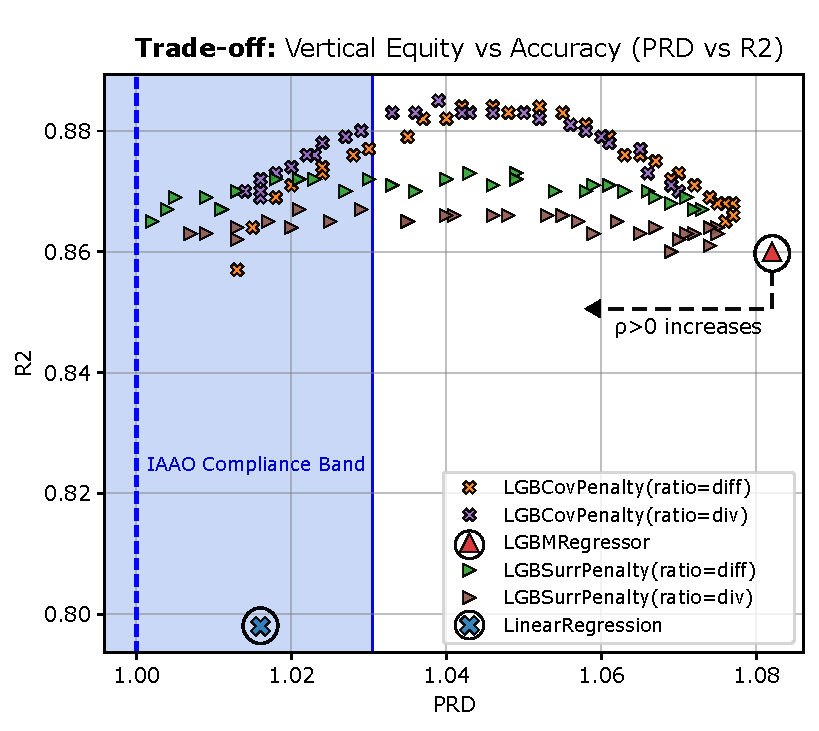
\includegraphics[width=\linewidth,trim={2mm 0 4mm 2mm}]{img/tradeoffs/PRD_vs_R2_band.pdf}}

\column{0.29\textwidth}
\begin{tcolorbox}[colback=Panel,colframe=LineGray,arc=1.5mm]
\textbf{Frontier logic}\\[1mm]
{\small Increasing $\rho$ traces candidate models, not a single universal winner.}
\end{tcolorbox}

\vspace{3mm}
\begin{tcolorbox}[colback=MethodBlue!6,colframe=MethodBlue!60,arc=1.5mm]
{\small The deployment question is which candidate satisfies assessor tolerances while keeping strong fit.}
\end{tcolorbox}
\end{columns}
\end{frame}

% ----------------------------------------------------------
% Slide 18
% ----------------------------------------------------------
\begin{frame}{Deployment rule: constrained calibration}
\begin{columns}[T,onlytextwidth]
\column{0.55\textwidth}
\centering
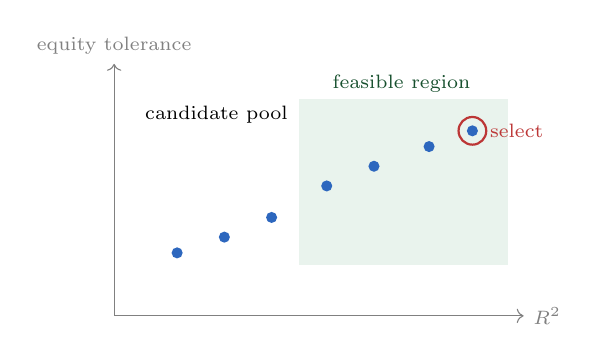
\begin{tikzpicture}[x=1cm,y=1cm]
  \draw[->,gray] (0,0) -- (5.2,0) node[right,font=\scriptsize] {$R^2$};
  \draw[->,gray] (0,0) -- (0,3.2) node[above,font=\scriptsize] {equity tolerance};
  \fill[Good!10] (2.35,0.65) rectangle (5.0,2.75);
  \node[Good!60!black,font=\scriptsize] at (3.65,2.95) {feasible region};
  \foreach \x/\y in {0.8/0.8,1.4/1.0,2.0/1.25,2.7/1.65,3.3/1.9,4.0/2.15,4.55/2.35} {
    \fill[MethodBlue] (\x,\y) circle (2pt);
  }
  \draw[Bad,thick] (4.55,2.35) circle (5pt);
  \node[Bad,font=\scriptsize,anchor=west] at (4.65,2.35) {select};
  \node[font=\scriptsize] at (1.3,2.55) {candidate pool};
\end{tikzpicture}

\column{0.42\textwidth}
\begin{tcolorbox}[colback=MITred!5,colframe=MITred!55,arc=1.5mm]
\textbf{Plain-English rule}\\[1mm]
Pick the best predictive candidate among models that meet the selected ratio-study tolerances.
\end{tcolorbox}

\vspace{3mm}
\begin{tcolorbox}[colback=Panel,colframe=LineGray,arc=1.5mm]
{\small This matches assessor practice: multiple diagnostics matter simultaneously, so final calibration is constrained rather than one-score ranking.}
\end{tcolorbox}
\end{columns}
\end{frame}

% ==========================================================
% Part V
% ==========================================================
\section{Closing}

% ----------------------------------------------------------
% Slide 19
% ----------------------------------------------------------
\begin{frame}{Main takeaway and honest scope}
\begin{columns}[T,onlytextwidth]
\column{0.48\textwidth}
\begin{tcolorbox}[colback=Good!6,colframe=Good!65,title=Takeaway,arc=1.5mm]
\begin{enumerate}
\item Stronger ML can worsen vertical equity.
\item A covariance-based penalty recovers much of the gap.
\item The surrogate is lightweight enough for assessor workflows.
\end{enumerate}
\end{tcolorbox}

\column{0.48\textwidth}
\begin{tcolorbox}[colback=Panel,colframe=LineGray,title=Scope,arc=1.5mm]
\begin{enumerate}
\item It does not directly optimize PRD, PRB, or VEI.
\item It gives no out-of-sample compliance guarantee.
\item It is global and first-order; local patterns can remain.
\end{enumerate}
\end{tcolorbox}
\end{columns}

\vspace{5mm}
\begin{center}
\textbf{Use the penalty as a correction layer, then choose the strongest feasible model.}
\end{center}
\end{frame}

% ----------------------------------------------------------
% Slide 20
% ----------------------------------------------------------
\begin{frame}[plain]
\vfill
\begin{center}
{\Huge\bfseries Questions?}\\[5mm]
{\footnotesize Implementation \quad Diagnostics \quad Deployment \quad Extensions}
\end{center}
\vfill
\end{frame}

% ==========================================================
% APPENDIX
% ==========================================================
\appendix
\section*{Appendix}

% ----------------------------------------------------------
% A1
% ----------------------------------------------------------
\begin{frame}{Appendix A1: Metric definitions}
\footnotesize
\[
r_i := \frac{AV_i}{MV_i}=\frac{\widehat{MV}_i}{MV_i},\qquad
\tilde r := \mathrm{median}(r),\qquad
\bar r := \frac{1}{n}\sum_i r_i,\qquad
\bar r_w := \frac{\sum_i MV_i r_i}{\sum_i MV_i}.
\]

\begin{columns}[T,onlytextwidth]
\column{0.48\textwidth}
\begin{tcolorbox}[colback=Panel,colframe=LineGray,title=Accuracy and dispersion,arc=1.5mm]
\[
R^2 = 1-\frac{\sum_i (MV_i-\widehat{MV}_i)^2}{\sum_i(MV_i-\overline{MV})^2},
\qquad
\mathrm{MAE}=\frac{1}{n}\sum_i|MV_i-\widehat{MV}_i|
\]
\[
\mathrm{COD}=100\cdot\frac{\frac{1}{n}\sum_i|r_i-\tilde r|}{\tilde r},
\qquad
\mathrm{COV}=\frac{\mathrm{SD}(r)}{\bar r}
\]
\end{tcolorbox}

\column{0.48\textwidth}
\begin{tcolorbox}[colback=Panel,colframe=LineGray,title=Vertical equity,arc=1.5mm]
\[
\mathrm{PRD}=\frac{\bar r}{\bar r_w}
\]
\[
\mathrm{PRB}=\mathrm{slope}\left(\frac{r_i-\tilde r}{\tilde r}\sim
\log_2\left(\frac{MV_i+AV_i/\tilde r}{2}\right)\right)
\]
\[
\mathrm{VEI}\approx100\cdot
\frac{\mathrm{median}(r)_{\text{top decile}}-\mathrm{median}(r)_{\text{bottom decile}}}{\tilde r}
\]
\end{tcolorbox}
\end{columns}
\end{frame}

% ----------------------------------------------------------
% A2
% ----------------------------------------------------------
\begin{frame}{Appendix A2: Up-to-date test-set results}
\tiny
\begin{center}
\resizebox{\textwidth}{!}{%
\begin{tabular}{lc|cc|cc|cc|ccc}
\toprule
Model Family & $\rho$ & $R^2$ & MAE & Med.\ $r$ & Mean $r$ & COD & COV & VEI & PRD & PRB \\
\midrule
Linear Regression & -- & 0.762 & \$86{,}257 & 1.001 & 1.051 & 25.013\% & 36.825\% & -13.474\% & 1.039 & -0.011 \\
LGBMRegressor & -- & 0.883 & \$72{,}064 & 0.944 & 1.021 & 23.106\% & 35.398\% & -36.816\% & 1.085 & -0.118 \\
\midrule
LGBSurrogatePenalty & 0.100 & 0.881 & \$73{,}272 & 0.936 & 1.011 & 23.125\% & 35.236\% & -36.367\% & 1.084 & -0.115 \\
LGBSurrogatePenalty & 0.189 & 0.881 & \$73{,}209 & 0.936 & 1.010 & 23.042\% & 35.048\% & -33.608\% & 1.080 & -0.107 \\
LGBSurrogatePenalty & 0.404 & 0.882 & \$73{,}111 & 0.937 & 1.006 & 22.924\% & 34.782\% & -29.878\% & 1.075 & -0.095 \\
LGBSurrogatePenalty & 0.761 & 0.883 & \$72{,}974 & 0.937 & 1.001 & 22.749\% & 34.189\% & -23.789\% & 1.067 & -0.076 \\
LGBSurrogatePenalty & 1.628 & 0.882 & \$73{,}233 & 0.938 & 0.994 & 22.645\% & 33.664\% & -16.431\% & 1.057 & -0.052 \\
LGBSurrogatePenalty & 3.070 & 0.881 & \$73{,}664 & 0.937 & 0.986 & 22.667\% & 33.620\% & -12.630\% & 1.048 & -0.032 \\
\textbf{LGBSurrogatePenalty} & \textbf{6.572} & \textbf{0.882} & \textbf{\$74{,}428} & \textbf{0.937} & \textbf{0.976} & \textbf{22.806\%} & \textbf{33.386\%} & \textbf{-8.545\%} & \textbf{1.038} & \textbf{-0.011} \\
LGBSurrogatePenalty & 12.390 & 0.879 & \$75{,}846 & 0.935 & 0.968 & 23.249\% & 33.684\% & -7.446\% & 1.032 & 0.003 \\
LGBSurrogatePenalty & 26.519 & 0.879 & \$77{,}114 & 0.933 & 0.960 & 23.719\% & 33.959\% & -4.484\% & 1.024 & 0.020 \\
LGBSurrogatePenalty & 50.000 & 0.878 & \$78{,}155 & 0.932 & 0.956 & 24.092\% & 34.336\% & -4.883\% & 1.021 & 0.027 \\
\midrule
LGBCovPenalty & 0.100 & 0.879 & \$73{,}459 & 0.937 & 1.014 & 23.210\% & 35.551\% & -38.368\% & 1.087 & -0.122 \\
LGBCovPenalty & 0.189 & 0.880 & \$73{,}312 & 0.939 & 1.015 & 23.221\% & 35.443\% & -37.671\% & 1.086 & -0.119 \\
LGBCovPenalty & 0.404 & 0.882 & \$72{,}947 & 0.941 & 1.017 & 23.224\% & 35.432\% & -36.501\% & 1.083 & -0.115 \\
LGBCovPenalty & 0.761 & 0.883 & \$72{,}608 & 0.944 & 1.019 & 23.157\% & 35.246\% & -34.017\% & 1.078 & -0.106 \\
LGBCovPenalty & 1.628 & 0.886 & \$72{,}198 & 0.949 & 1.023 & 23.176\% & 35.086\% & -30.427\% & 1.071 & -0.096 \\
LGBCovPenalty & 3.070 & 0.884 & \$72{,}294 & 0.955 & 1.027 & 23.216\% & 35.053\% & -26.850\% & 1.065 & -0.085 \\
LGBCovPenalty & 6.572 & 0.881 & \$72{,}872 & 0.961 & 1.030 & 23.282\% & 35.040\% & -20.525\% & 1.055 & -0.068 \\
LGBCovPenalty & 12.390 & 0.878 & \$73{,}449 & 0.963 & 1.030 & 23.261\% & 34.757\% & -16.050\% & 1.048 & -0.057 \\
LGBCovPenalty & 26.519 & 0.870 & \$74{,}742 & 0.963 & 1.028 & 23.310\% & 34.542\% & -13.572\% & 1.041 & -0.046 \\
LGBCovPenalty & 50.000 & 0.866 & \$75{,}575 & 0.960 & 1.023 & 23.357\% & 34.522\% & -11.105\% & 1.037 & -0.039 \\
\bottomrule
\end{tabular}}
\end{center}
\smallnote{Canonical source: latest paper table. The main deck uses the surrogate at $\rho=6.572$ as the operational headline.}
\end{frame}

% ----------------------------------------------------------
% A3
% ----------------------------------------------------------
\begin{frame}{Appendix A3: Penalty formulas and implementation}
\footnotesize
\begin{columns}[T,onlytextwidth]
\column{0.49\textwidth}
\begin{tcolorbox}[colback=Panel,colframe=LineGray,title=Direct squared covariance,arc=1.5mm]
\[
\Psi_{\mathrm{cov}}(f)
=\widehat{\Cov}(e(f),y)^2
=\left(\frac{1}{n}\sum_i(e_i-\bar e)(y_i-\bar y)\right)^2.
\]
Conceptually exact for first-order dependence control, but non-separable across observations.
\end{tcolorbox}

\column{0.49\textwidth}
\begin{tcolorbox}[colback=MethodBlue!6,colframe=MethodBlue!65,title=Separable surrogate,arc=1.5mm]
\[
\Psi_{\mathrm{surr}}(f)
=\frac{1}{n}\sum_{i=1}^n e_i(f)^2\,(y_i-\bar y)^2.
\]
Sample-additive, with per-observation weights fixed before training.
\end{tcolorbox}
\end{columns}

\vspace{3mm}
\begin{tcolorbox}[colback=Good!6,colframe=Good!60,arc=1.5mm]
\centering
For squared loss plus surrogate penalty, the custom objective contributes per-observation gradient and Hessian terms proportional to $(1+2\rho(y_i-\bar y)^2)e_i$ and $1+2\rho(y_i-\bar y)^2$.
\end{tcolorbox}
\end{frame}

% ----------------------------------------------------------
% A4
% ----------------------------------------------------------
\begin{frame}{Appendix A4: Formal constrained calibration}
\footnotesize
\begin{tcolorbox}[colback=Panel,colframe=LineGray,arc=1.5mm]
Let $c\in\mathcal{C}$ index candidate configurations and $v\in\mathcal{V}$ index validation folds. For each $(c,v)$, compute prediction error $\mathcal{E}_v(c)$ and diagnostics $\mathcal{F}_{m,v}(c)$.
\[
c^*\in\argmin_{c\in\mathcal{C}}\frac{1}{|\mathcal{V}|}\sum_{v\in\mathcal{V}}\mathcal{E}_v(c)
\quad
\mathrm{s.t.}\quad
\mathcal{F}_{m,v}(c)\le \tau_m,\quad \forall m,\;v.
\]
\end{tcolorbox}

\begin{columns}[T,onlytextwidth]
\column{0.48\textwidth}
\begin{itemize}
\item Recommended default when tolerances are known.
\item Equivalent to choosing the strongest predictive feasible candidate.
\item Add PRD, PRB, VEI, COD, COV, or ratio guardrails.
\end{itemize}

\column{0.48\textwidth}
\centering
\figurebool{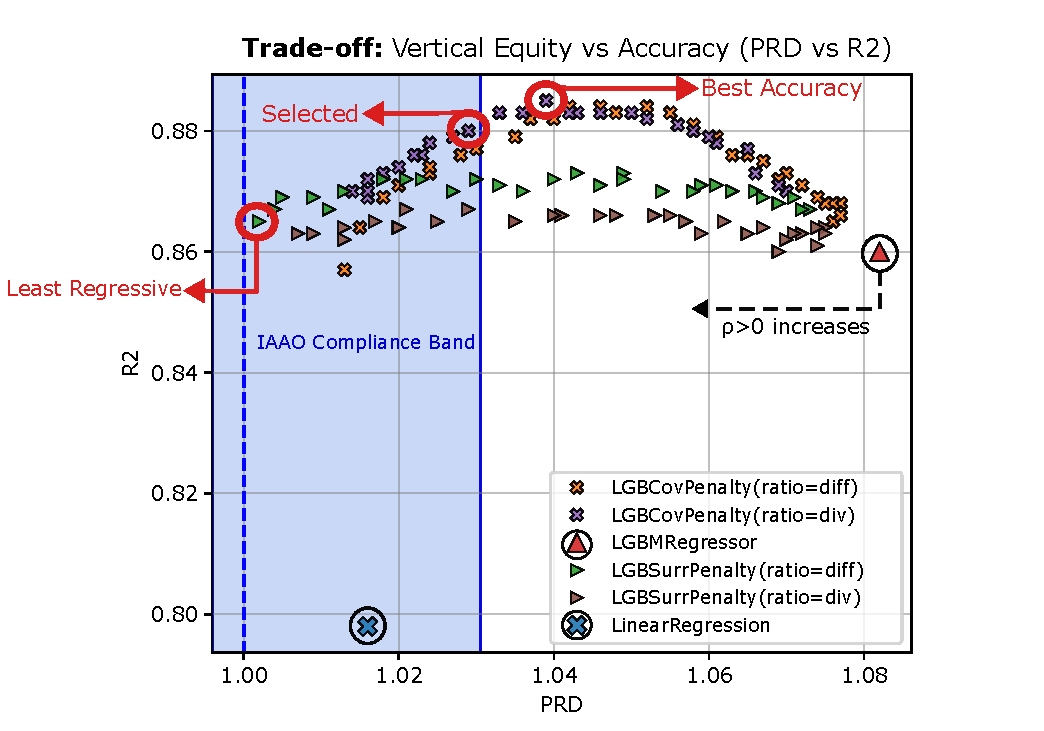
\includegraphics[width=0.92\linewidth,trim={2mm 2mm 4mm 4mm}]{img/model_selection/pareto_optimal.pdf}}
\end{columns}
\end{frame}

\begin{frame}{Appendix A4: Selection criteria on the test set}
\tiny
\begin{center}
\resizebox{0.95\textwidth}{!}{%
\begin{tabular}{llc|cc|cc|cc|ccc}
\toprule
Solution & Model & $\rho$ & $R^2$ & MAE & Med.\ $r$ & Mean $r$ & COD & COV & PRD & PRB & VEI \\
\midrule
\multicolumn{12}{l}{\textbf{Unconstrained baselines}} \\
BASELINE & Linear Reg. & -- & 0.762 & \$86{,}257 & 1.001 & 1.051 & 25.01\% & 36.83\% & 1.039 & -0.011 & -13.47\% \\
BASELINE & LGBM & -- & 0.883 & \$72{,}064 & 0.944 & 1.021 & 23.11\% & 35.40\% & 1.085 & -0.118 & -36.82\% \\
\midrule
\multicolumn{12}{l}{\textbf{Constraints: PRD}} \\
CONSTRAINED & LGBSurrogate & 5.96 & 0.881 & \$74{,}416 & 0.937 & 0.978 & 22.80\% & 33.64\% & 1.039 & -0.014 & -9.27\% \\
UTOPIA & LGBSurrogate & 100.00 & 0.877 & \$79{,}217 & 0.930 & 0.953 & 24.47\% & 34.89\% & 1.019 & 0.032 & -4.41\% \\
NASH & LGBSurrogate & 2.95 & 0.883 & \$73{,}395 & 0.938 & 0.988 & 22.63\% & 33.63\% & 1.048 & -0.034 & -12.20\% \\
\midrule
\multicolumn{12}{l}{\textbf{Constraints: PRD, PRB, and VEI}} \\
CONSTRAINED & LGBSurrogate & 5.96 & 0.881 & \$74{,}416 & 0.937 & 0.978 & 22.80\% & 33.64\% & 1.039 & -0.014 & -9.27\% \\
UTOPIA & LGBSurrogate & 7.91 & 0.882 & \$74{,}939 & 0.935 & 0.974 & 23.02\% & 33.85\% & 1.036 & -0.007 & -8.36\% \\
NASH & LGBSurrogate & 5.96 & 0.881 & \$74{,}416 & 0.937 & 0.978 & 22.80\% & 33.64\% & 1.039 & -0.014 & -9.27\% \\
\midrule
\multicolumn{12}{l}{\textbf{Constraints: PRD, mean ratio, and COD}} \\
INFEASIBLE & -- & -- & -- & -- & -- & -- & -- & -- & -- & -- & -- \\
UTOPIA & LGBSurrogate & 6.87 & 0.882 & \$74{,}449 & 0.937 & 0.977 & 22.84\% & 33.72\% & 1.038 & -0.011 & -9.38\% \\
NASH & LGBSurrogate & 2.95 & 0.883 & \$73{,}395 & 0.938 & 0.988 & 22.63\% & 33.63\% & 1.048 & -0.034 & -12.20\% \\
\midrule
\multicolumn{12}{l}{\textbf{Constraints: full metric set}} \\
INFEASIBLE & -- & -- & -- & -- & -- & -- & -- & -- & -- & -- & -- \\
UTOPIA & LGBSurrogate & 5.96 & 0.881 & \$74{,}416 & 0.937 & 0.978 & 22.80\% & 33.64\% & 1.039 & -0.014 & -9.27\% \\
NASH & LGBSurrogate & 5.96 & 0.881 & \$74{,}416 & 0.937 & 0.978 & 22.80\% & 33.64\% & 1.039 & -0.014 & -9.27\% \\
\bottomrule
\end{tabular}}
\end{center}
\end{frame}

% ----------------------------------------------------------
% A5
% ----------------------------------------------------------
\begin{frame}{Appendix A5: Additional frontier diagnostic}
\begin{columns}[T,onlytextwidth]
\column{0.68\textwidth}
\centering
\figurebool{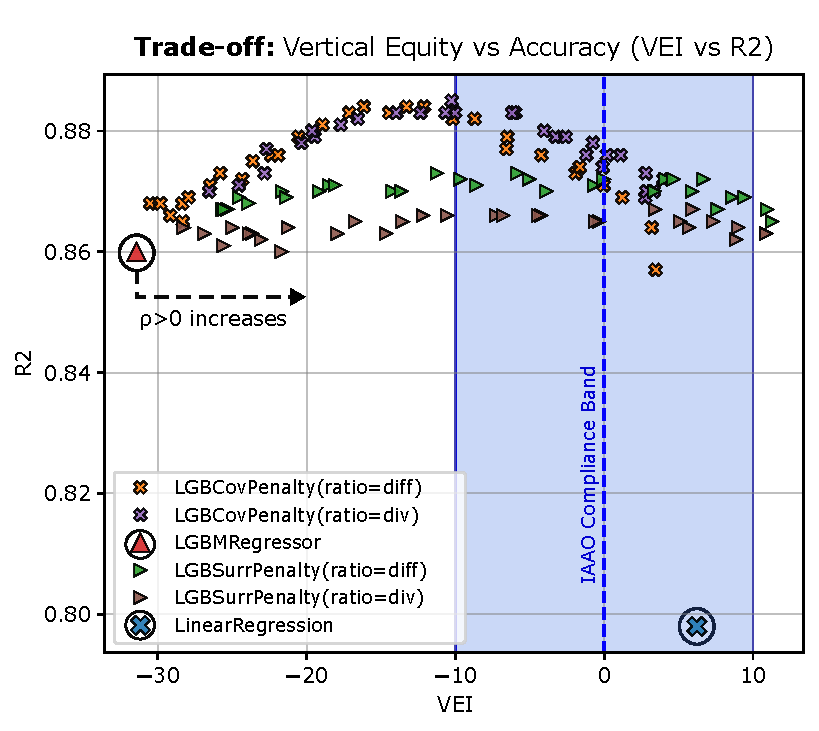
\includegraphics[width=\linewidth,trim={4mm 0 0 2mm}]{img/tradeoffs/VEI_vs_R2_band.pdf}}

\column{0.29\textwidth}
\begin{tcolorbox}[colback=Panel,colframe=LineGray,arc=1.5mm]
{\small The same frontier logic appears in VEI-$R^2$ space: penalized models move toward the vertical-equity band while staying close to the accuracy frontier.}
\end{tcolorbox}
\end{columns}
\end{frame}

\begin{frame}{Appendix A6: Correlation evolution across $\rho$}
\centering
\figurebool{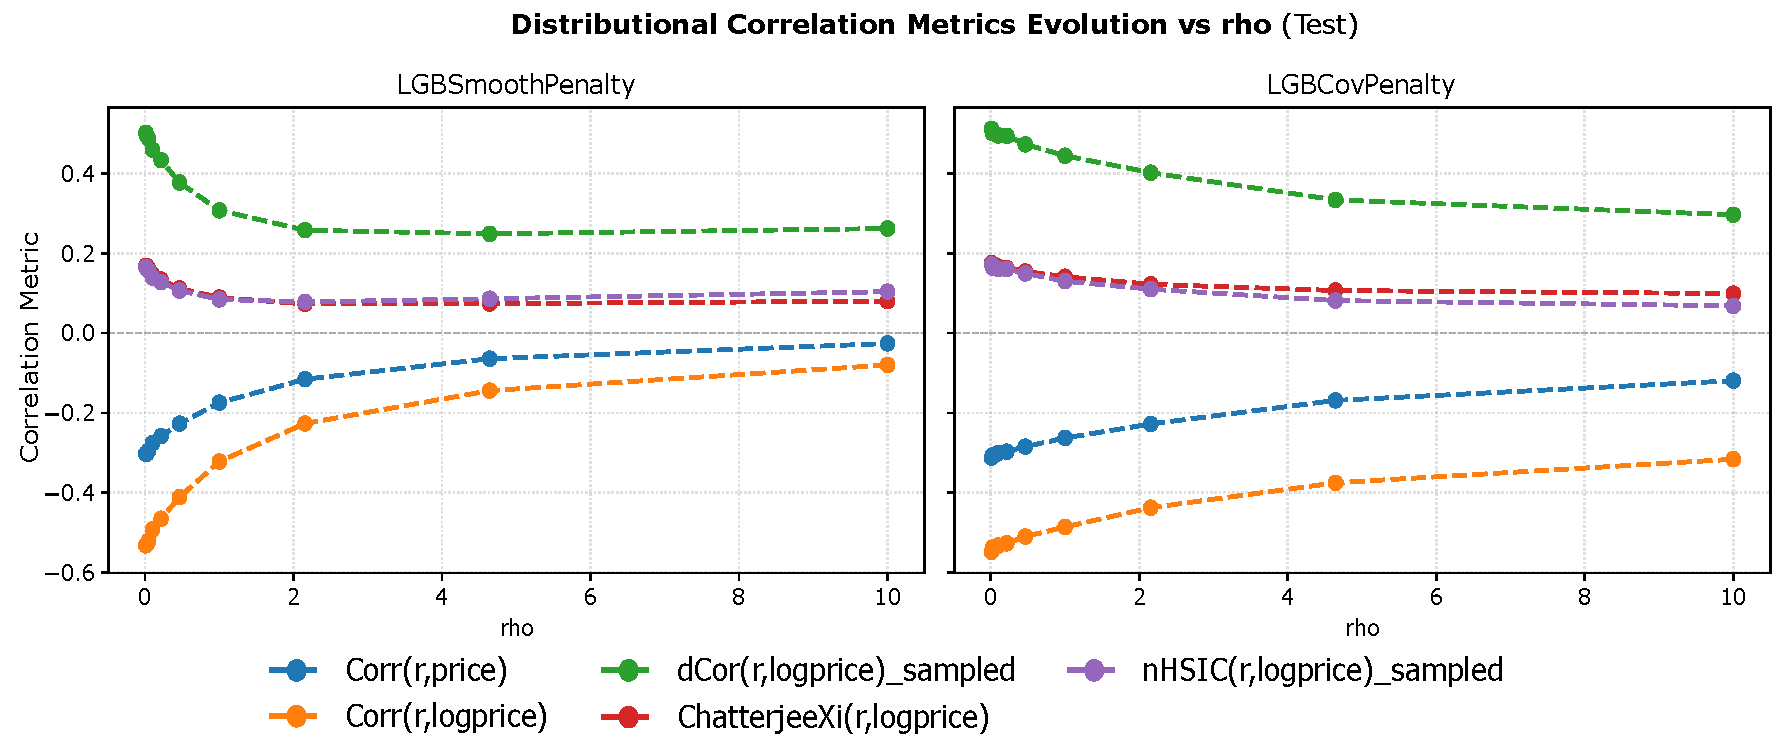
\includegraphics[width=0.9\linewidth]{img/correlations/correlations.pdf}}

\vspace{1mm}
\smallnote{Residual-price and ratio-price correlations move toward zero as the penalty strength increases.}
\end{frame}

\end{document}
